\documentclass[colorlinks]{thesis-ekf}
\usepackage[T1]{fontenc}
\usepackage[utf8]{inputenc}
\PassOptionsToPackage{defaults=hu-min}{magyar.ldf}
\usepackage[magyar]{babel}
\usepackage{graphicx,amsmath,amssymb,amsthm}
\graphicspath{{./figures/}} % A képfájlokat a [figures] mappába kell tenni!
\footnotestyle{rule=fourth}

\newtheorem{tetel}{Tétel}[chapter]
\newtheorem{lemma}[tetel]{Lemma}
\theoremstyle{definition}
\newtheorem{definicio}[tetel]{Definíció}
\newtheorem{feladat}[tetel]{Feladat}
\theoremstyle{remark}
\newtheorem{megjegyzes}[tetel]{Megjegyzés}
\newtheorem*{megoldas}{Megoldás}

\begin{document}
\logo{
\includegraphics[width=9cm]{eke-logo}}
\institute{Matematikai és Informatikai Intézet}
\title{Chemist \\ Kémiai Legó}
\author{Fehér Rózsa Zsuzsanna\\ Programtervező Informatikus Bsc}
\supervisor{Troll Ede \\Tanársegéd}

\city{Eger}
\date{2019}
\maketitle
\tableofcontents

\chapter{Bevezetés}
Szakdolgozatom témája egy Unity-ban megírt háromdimenziós ismeretterjesztő játék, ahol a Mengyelejev tábla elemei közül különféle atomokat kiválasztva molekulákat, ionokat és fémes kötéseket hozhatunk létre.
A játék célkorosztálya első sorban az általános iskolások korcsoportja. Így főként ezekben az időkben tanult kémiai kötések, atomok és molekulák felépítését szemlélteti a játék a modelleken keresztül.

A szoftver alapvetően drag and drop technológián alapul, ezért is, illetve, mert a játékfelületen törölni és mozgatni lehet a molekulákat és atomokat javasolt az egér használata.

Választásom azért esett erre a témára, mivel jómagam is nehezen tudtam elképzelni ezeket kötéseket általános iskolásként, valamint érdekelt a háromdimenziós modellezés és játékfejlesztés is. Így a Unity-vel lehetőségem volt közelebbről megismerkedni a játékfejlesztéssel magával, illetve a modellezés lépéseivel, valamint a kémiai háttér tudásom is gyarapodott.
%
A szakdolgozat részletezni fogja a technológiát, illetve összehasonlítja más fejlesztőkörnyezetekkel. Ismertetni fogja, hogy milyen kémiai ismeret volt szükséges a szoftver elkészítéséhez, valamint bemutatásra kerül maga a játék is az azokban használt modellekkel, és felhasználói interakció lehetőségekkel együtt. 

Mivel a témakör elég tág, illetve az oktató játék csak szűkös tudományos forrással készült, ezért a továbbfejlesztési lehetőségek akár több irányban is folytatódhatnak.

\chapter{Kémia az iskolákban}
A kémia oktatása, mint minden egyéb természettudományos tárgyé más kihívásokat rejt, mint a humán tárgyaké. 

A természet tudománnyal fogalakozó tárgyakat, így a kémiát is kétféleképpen lehet megközelíteni oktatás szempontjából. Induktív és deduktív módon. 

Induktív módszernél egy konkrét természeti jelenségből indulunk ki,
amelyet kísérlettel modellezünk, ezt értelmezzük, majd általánosítjuk. Míg a deduktívnál egy hipotézist igyekszünk bizonyítani például egy kísérlettel. De mindkettőben  fontos szerepet játszik a kísérletezés, illetve a vizualizáció. A vizualizációban pedig a modellek használata. \cite{kémia_modertan}

Az a jó modell ami a láthatatlant, nehezen elképzelhetőt segít elképzelni. Elég egyszerűnek kell lennie, hogy megértsük, átlássuk, viszont realisztikusnak kell lennie ahhoz, hogy tükrözze a valóságot bizonyos aspektusból, így könnyebben összevethető azzal. \cite{kémia_modertan}

Kémia oktatásában a szemléltethető eszközöket két nagy csoportra lehet osztani. Az egyik az Eugon vagy kalott modell, ami csonkolt gömbökből áll, jól szemléltetve a molekula térkitöltését, míg a másik a pálcika vagy vázmodell. Ezen kis gömbök vagy hengerek találhatók, amelyeken egy vagy több csap helyezkedik el. Ez utóbbiak a vegyértékhéjnak tekinthetők. A csapok száma és az egymással bezárt szögeik a kötésorientációkat jelzik. \cite{kémia_modertan}

Az idomok színezése mindkét fajtánál a nemzetközi szabvány szerint történik. Fehér jelenti a hidrogénatomot, piros az oxigénatomot, míg a fekete a szénatom, a zöld a klóratom, a sárga a kénatom, a pedig kék a nitrogénatomot reprezentálja. A pálcikamodell-készletben esetében még találhatók bizonyos színű csövek is a kötések kialakításához. Célszerű következetesen a zöld csöveket a szigma, a fehéreket a pí kötések jelzésére használni. \cite{kémia_modertan}

Ezek a szemléltető eszközök azon kívül,hogy tükrözik hány nemkötő elektron párja van a vegyületnek, a molekulát alkotó elemek egymáshoz viszonyított helyzetét, alakját, távolságát. Fő céljuk a vegyület térszerkezetének bemutatása, ami összetettebb molekulák esetén eléggé bonyolult térszerkezetet eredményez. Az ilyen modellek segítségével viszont könnyebben lehet fejleszteni a diákok térlátását, mind egy kétdimenziós rajz segítségével.\cite{kémia_modertan}

Innen jött az ötlet, hogy a játék ezen modellek felhasználásával reprezentálja a kötéseket három dimenzióban. Ez a megkötés főleg a kovalens kötésnél volt fontos. 

Már most is rengeteg molekula s vegyület modellező szoftver létezik a piacon. Általában molekula szerkesztőknek nevezik őket. Ezek olyan számítógépes programok, amik kémiai szerkezetek létrehozására, módosítására használatosak. Ezek képesek az ábrázolt kémiai szerkezetek megváltoztatására mind 2D , mind 3D  szimulált környezetben. A kétdimenziós kimenetek illusztrációként vagy adatbázisban való kereséshez használatosak. A háromdimenziós kimenetek, pedig molekulamodellek építésére használhatóak, általában molekulamodellező szoftverek részeként.
Adatbázisszerű molekula szerkesztők, úgy mint a Leatherface\cite{Leather} és RECAP\cite{recap} megengedik a nagy számú molekulák automatikus változtatását a felhasználó által.
Jellemzően támogatják a modell valamilyen fájlba való írását és olvasását is. 
\cite{molekula_editorok}

Jó példa ezen szoftverekre az ACD/ChemSketch. Ez egy olyan interfész, amely képes létrehozni illetve módosítani kémiai kötéseket. Az ACD/LAbs azaz Advanced Chemistry Development, Inc által készített ingyenes program, ami Windows operációs rendszerre elérhető.  A program kettő illetve három dimenzióban is képes a vegyületek szerkezetét megjeleníteni, forgatni. Szinekkel és különböző feliratokkal lehet ellátni a vegyületek alkotóelemeit. Ezen kívül tartalmaz sok ion és molekula sablonokat, feliratozási lehetőségekkel is.\cite{wiki_ACD}

Ehhez hasonló program a ChemDrawPro, ami viszont már nem érhető el ingyenesen. A PerkinElmer által fejlesztet program. Két dimenzióban dinamikusan lehet kötéseket létrehozni/rajzolni. Főleg kutatók használják fejlett és professzionális funkciói miatt. (adatelemzés, dinamikus vegyület rajzolás stb.)\cite{ChemDraw}

De a teljesség értéke nélkül még léteznek online szerkesztők is.

Ilyen például a PubChem, ez is két dimenzióban rajzolja ki a kötéseket a ChemDrawhoz hasonlóan. Viszont emellett a világ legnagyobb ingyenesen hozzáférhető kémai adatbázisa is jelenleg. A rajzoló felülete inkább gyors vázlatokra, illetve kutatási publikációkban használt rajzok elkészítéséhez ajánlott. \cite{PubChem}

%Milyen egyébb kötéseket reprezzentáló program lézetik, és azok hogyan működnek

\chapter{Kémiai háttér}

A játék működéséhez elengedhetetlen az atom felépítésének és a kötések kialakulásának ismerete. 
\section{Atomok}
Mint tudjuk az atomok protonokból, neutronokból és elektronokból állnak. A protonok töltése pozitív, az elektronoké negatív, a neutronok töltését pedig tekintsük szemlegesnek. Az elektronokon kívül a nukleonok az atom magjában található, míg az elektronok az atom mag körül ''keringenek,, előre meghatározott elektronpályákon.

Ezek az elektronpályák kisebb pályákból/ héjakból állnak. Minden ilyen nagyobb pályán megtalálhatók ezek az al héjak ha az atom rendelkezik megfelelő számú elektronnal. Ezeken az al héjakon meghatározott számú elektron foglalhat helyet.Az s pályán 2 elektron, a p pályán 6 elektron, a d pályán 10 elektron, illetve az f pályán 12 elektron fér el.\cite{sulinet_elektronpályák}
\begin{figure}[!ht]
	\centering
	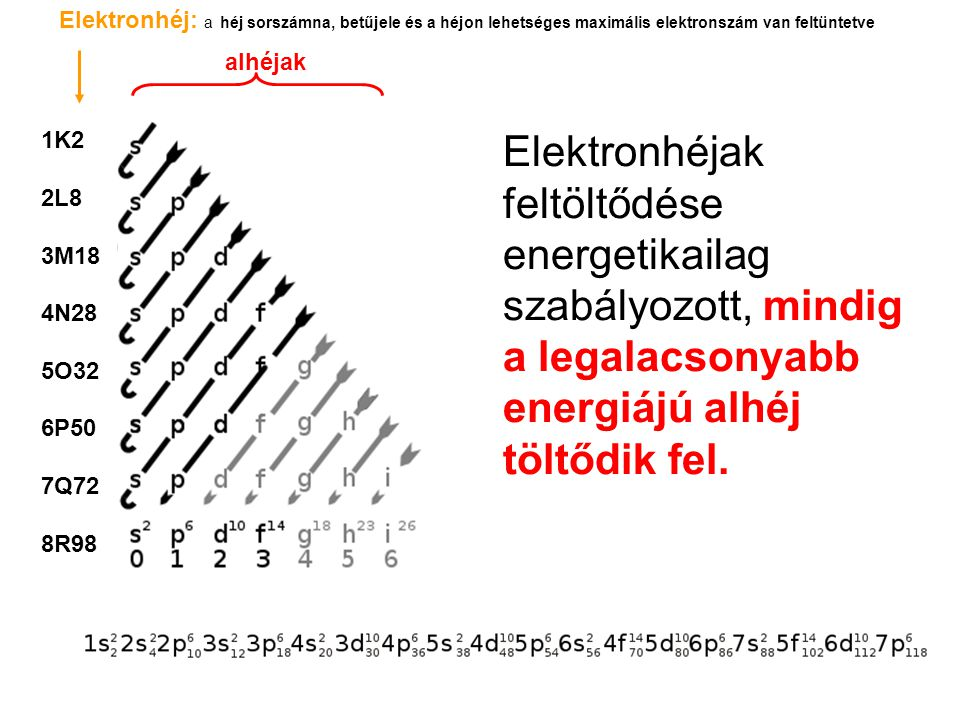
\includegraphics[width=9cm]{elektronszerkezet}
	\caption{\cite{img_elektronkonfig}}\label{elektronszerkezet}
\end{figure}

Mivel az atomok szabad állapotban a természetben ritkán fordulnak elő (kivéve a nemesgázok stabil szerkezetük miatt), fontos a kémia kötésekről beszélnünk, ugyanis csak is ezek a reakciók teszik lehetővé azt, hogy a periódusos rendszerbeli elemek elérjék a kívánt stabil(nemesgázbeli) állapotukat. Ezt úgy teszik, hogy más atomokkal különböző kötéseket létesítenek.\cite{ionos_vidi} De mégis mi határozza meg azt, hogy milyen kötés alakul ki két szabad atom között?

Az atomokban és molekulákban lévő elektronok elhelyezkedése, azaz az elektronszerkezet, határozza meg az atomok és molekulák kémiai viselkedését.\cite{wiki_e_szerk}
Azokat az anyagokat, amik ugyanolyan rendszámú (azaz azonos mennyiségű elektronnal rendelkező) atomokból épülnek fel, kémiai elemeknek hívjuk, és vegyjellel hivatkozunk rájuk.\cite{periodusos_ppt} 

A későbbiek folyamán az atom megnevezést a kémiai elemekre fogom használni. A szoftver szempontjából a kettőt egyformának tekinthetjük.

Az elektronszerkezeten belül, az elektronkonfiguráció, és azon belül a legkülső héj elektronkonfigurációja valamint az ahhoz kapcsolódó vegyérték elektronok, illetve az elektronegativitás játszik szerepet abban, hogy egy atom milyen kötést tud létesíteni más atomokkal. 

Kémiai kötésnek nevezzük azt, amikor több atom reakcióba lépése során egy közös, stabil (telített) külső elektronhéj alakul ki.Ezek lehetnek elsőrendű és másodrendű kémiai kötések. A kovalens, ionos és fémes kötés az elsőrendű kötések közzé tartozik\cite{miskolc_kemia}, valamint a játék is csak ezekkel a kötésekkel foglalkozik.

Az elektronkonfiguráció az elektronok pályák szerinti elrendeződését írja le egy atomban.\cite{periodusos_ppt} Mivel az elektronpályák nem expliciten töltődnek fel, hanem az al héjak energiaszintjének megfelelően, így sokszor előfordul, hogy egy elektronpálya (elektronhéj) még nem telítődik meg, de már az eggyel nagyobb héjon észlelhetünk elektronokat.(Lásd \aref{elektronszerkezet}.~ábrán)
A legkülső elektronhéjat szokás vegyértékhéjnak nevezni, míg az ezen tartózkodó elektronokat vegyértékelektronoknak.\cite{vegyérték_sulinet} Ezek közül kerülnek ki azok az elektronok, amik képesek kötéseket kialakítani (vegyértéke), illetve ionos kötésnél a vegyérték elektronok száma határozza meg azt, hogy ők adják-e át a másik atomnak az elektronjaikat, vagy ők veszik el.\cite{ionos_vidi}

Ha a maximális vegyértékeket nézzük a periódusos táblában az egy oszlopon belül változhat. A felsőbb periódusokban az elemek rendszerint kevesebb vegyértékelektronnal képesek kötést létesíteni, mint az alsóbb periódusokban található elemek.\cite{periodusos_ppt}De általánosan a vegyértéke elektronok számát a periódusos rendszerből könnyen meglehet állapítani, ugyanis a táblázat oszlopai fölötti számokat kell nézni.(Főcsoportokat) \cite{vegyérték_sulinet}

Az elektronegativitás(EN) olyan mennyiség, ami azt írja le, hogy mekkora elektrosztatikus erő hat a másik atom vegyértékelektronjaira.\cite{angol_en} Értékét Slater szabállyal, illetve az empirikus megfigyeléseken alapuló Pauli elektronegativitási rendszerrel lehet meghatározni. Utóbbiban az atomokhoz tartozó elektronegativitásokat a lítiumhoz és fluorhoz képest viszonyították. Mivel viszonyszám, mértékegysége nincs.\cite{miskolc_kemia}\cite{eke_kemia_ppt}

\begin{figure}[!ht]
	\centering
	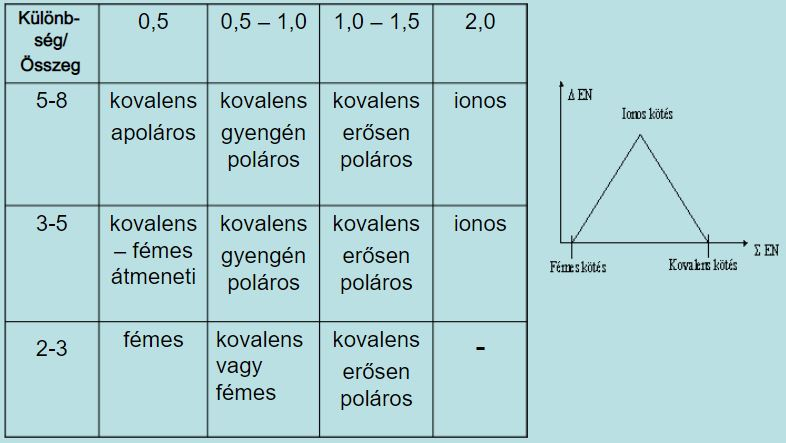
\includegraphics[width=9cm]{en_slide}
	\caption{\cite[52.~ppt]{periodusos_ppt}}\label{EN_tablazat}
\end{figure}
\Aref{EN_tablazat}.~ábrán látható, hogy milyen kötések alakulhatnak ki az elektronegativitástól függően, ahol a \begin{math}\Delta EN\end{math} a két atom elektronegativitásai között különbséget, míg \begin{math}\Sigma EN\end{math} az összeget jelöli.\cite{eke_kemia_ppt}
\section{Ionos kötés}

Ionos kötésnél két ionizált atom között lép fel elektrosztatikus vonzás.
Atomból ion úgy alakulhat ki, hogy az atommal közölnek egy bizonyos mennyiségű energiát. Ez az ionizációs energia. 

Definíció szerint az ionizációs energia, nem más, mint az az energiamennyiség  amely az n-edik elektron leszakításához szükséges, miután az előző n–1-et már leszakítottuk.\cite{miskolc_kemia}
Ilyenkor a nagyobb elektronegativitással rendelkező atom elektronokat vesz el a kisebb elektronegativitású atom vegyértékelektron héjáról, viszont a két atom teljes egybeolvadását az alacsonyabb elektronhéjak taszító hatása megakadályozza.\cite{miskolc_kemia}

Az, hogy hány elektront tud leszakítani, illetve hányat képes befogadni az ion attól függ, hogy milyen messze van a nemesgáz konfigurációtól.

Nemesgáz konfiguráció alatt az értjük, amikor az elektronszerkezet a legstabilabb. Gyakorlatban ez azt jelenti, hogy a vegyértékhéjon nyolc vegyérték elektron van, azaz telítve van.\cite{ionos_vidi}

Tehát ha vennénk két atomot,melyeknek elektronegativitásuk közötti különbség legalább kettő (Lásd \aref{EN_tablazat}.~ábra), akkor az egyik atommagja elkezdi vonzani a másik atom elektronjait, és ugyanezt teszi a másik is, így közeledve egymáshoz. Végül a nagyobb \begin{math} EN\end{math}-el rendelkező atom húzná el a másik vegyérték elektronjait. De abból is csak annyit, hogy ő maga, illetve a másik atom is nemesgáz konfigurációba kerüljön. \cite{ionos_vidi}

Érdemes azt is szem előtt tartani, hogy képlet szempontjából az ionos és kovalens kötésben lévő vegyületek és molekulák képletei hasonlóan néznek ki, de ionos kötésnél a számok, nem tényleges mennyiségeket jelölnek, hanem csupán arányokat.\cite{ionos_vidi}
\section{Fémes kötés}

Fémes kötés során több kevés vegyérték elektronnal rendelkező, illetve kis elektronegativitású atomok kapcsolódnak. Az alacsony elektronegativitás oka az lehet, hogy ezeknél az atomoknál a vegyértékelektronok elég távol helyezkedek el az atomtól, így elektronegativitásuk, és ionizációs energiájuk is kisebb. Mivel \begin{math}\Delta EN\end{math} és \begin{math}\Sigma EN\end{math} is kicsi, ezért olyan kötés jön létre, amelyben a vegyértékelektronok a kötésben valamennyi fématomhoz tartoznak, ezt nevezzük delokalizált elektronrendszernek.\cite{miskolc_kemia}

Azaz nincsenek különálló molekulák, sem szabad atomok, hanem a leglazábban kötött elektronok a fématomokról leszakadva valamennyi visszamaradt fémionhoz közösen tartoznak.\cite{eke_kemia_ppt}. Szilárd halmazállapotban ezek a lazán kötött atommagok és a közös elektronfelhőjük fémrácsokat alkotnak. A rácsszerkezeten belül az elektronok könnyen tudnak vándorolni, ezért is jól vezetik a fémek az elektromosságot, illetve a hőt.\cite{wiki_femes} Valamint a rács szerkezet síkjai is könnyen eltudnak gördülni egymáson, emiatt lehet a fémeket aránylag egyszerűen megmunkálni.

\section{Kovalens kötés}\label{kovalens}
Kovalens kötés során a két atom egy vagy több elektronpárral kötődnek egymáshoz.\cite{eke_kemia_ppt} Ez a legerősebb kötési forma, főleg ha a kötés folyamén stabil molekula alakul ki, ugyanis ekkor az elektronpárok egy úgynevezett közös molekulapályára kerülnek\cite{miskolc_kemia}, amik az atompályák átfedéséből keletkeznek.\cite{eke_kemia_ppt}

Azok az elektronok, amik leszakadnak a vegyértékhéjról, majd azután a kötésben részt vesznek és párokat alkotnak kötő elektronpároknak hívják, a kötésben részt nem vevő elektronokat pedig nem kötő elektronoknak illetve elektronpároknak hívják.\cite{eke_kemia_ppt}

 Azt, hogy ezen a közös molekulapályán hogyan viselkednek az elektronok, illetve a pályák hogy alakulnak ki, azt kvantumelmélet pár szabálya írja le. \cite{miskolc_kemia}
 \begin{itemize}
 	\item \textbf{Energiaminimum elve}: Ez mondja meg, hogy az elektronok mindig a lehető legalacsonyabb energiaszintre akarnak kerülni, ezért ha lehetséges a legalacsonyabb energiája elektronpályák telnek be. Valamint ha valaminek kisebb az energiaszintje, az annál stabilabb, ezért minél kisebb az energiaszintje a molekula pályának annál stabilabb, tehát erősebb. \cite{miskolc_kemia}
 	\item \textbf{Pauli elv}: Az elektronok nem lehetnek ugyanabban az állapotban, ez azt a jelentést hordozza magával, hogy a molekulapályákon legfeljebb két elektron helyezkedhet el, amiknek a spinje ellentétes.\cite{miskolc_kemia} (Ez a törvény nem csak a molekulapályára érvényes)
 	\item \textbf{Hund szabály}: Azonos energiájú pályák betöltése élészőr a párosítatlan elektronokkal történik. \cite{miskolc_kemia}
 \end{itemize}

A kovalens kötésnél fontos a létrejött molekulának geometriai felépítése, ugyanis ez jelentősen befolyásolja az adott anyag kémiai viselkedését. Egyik erre vonatkozó elmélet a Lewis-Kössel elmélet. Ez arról szól, hogy a kötésben lévő atomok vegyértékelektronjai nemesgáz konfigurációra törekednek.Emiatt több egymástól különböző kötés típusokat tudunk megkülönböztetni.

Az egyik ilyen a szigma kötés. Ekkor a két atommagot összekötő egyenesre forgásszimmetrikus a kötés. Létrejöhet két s, s és p illetve ha teljesíti a geometriai feltételt két p és p, hibrid pályák között is. Mivel a legalacsonyabb energiapályákról származnak a kötőelektronok (s), ezért ez a legerősebb, valamint minden kovalens kötésben van szigma kötés.

A másik kötésfajta a pí kötés. Ez a kötés alapvetően a p pályákon lévő kötőelektronok között jön létre, de ha a geometriai orientációja megfelelő, akkor akár két d héj között is kialakulhat. Mivel a kötő elektronok magasabb energiaszintű pályákról származnak, ezért ez a kötés gyengébb, mint a szigma kötés.\cite{miskolc_kemia} Nem forgásszimmetrikus, hanem a kötésre merőleges a kötés.\cite{eke_kemia_ppt}

Mivel a kovalens kötés több elektronpár között is kialakulhat.Lehetnek egyszeresek, kétszeresek illetve háromszorosak is. Egyszeres kötésnél a kötést csak egy szigma alkotja, a kettős kötésnél két elektronpár alakít ki egy szigma és egy pí kötést. A hármas kötést mindig három elektronpár alakítja ki, amelyek közül az egyik elektronpár egy szigma kötést hoz létre, míg a másik kettő két pí kötést.\cite{eke_kemia_ppt}

Ezek a kötések térbeli helyzetei határozzák meg a molekula tényleges alakját. A geometriai alakhoz tartozik a kötésszög illetve a kötéstávolság. 

Kötéstávolság a két kötő atom atommagjának távolsága a molekulában. Minél több kötés jön létre a távolság annál kisebb lesz. A kötésszög a kapcsolódó atomok által bezárt szög, azaz atommagot gondolatban összekötő egyeneséhez képest. \cite{eke_kemia_ppt}
\chapter{Unity és a fejlesztői lehetőségek}
%min 2 oldal
A játék elkészítése előtt el keltet döntetni, hogy milyen nyelven és milyen fejlesztőkörnyezet segítségével írjuk meg a szoftvert. Mivel mindenképp háromdimenziós modellezés szükséges, valamint könnyű, látványos és dinamikus felületet szerettünk volna, így egyértelművé vált, hogy olyan programnyelvet kellet keresni, amivel egyszerűen lehet kezelni különféle objektumokat, amiknek más és más tulajdonságai vannak. Azaz mindenféleképpen olyan nyelvet kellet választani, amiben az objektum orientáltságot hatékonyan lehet implementálni. Ezzel ki lett zárva a C, Basic, valamint a különféle script nyelvek, mint a Python is. A C++ támogatja az objektum orientáltságot, viszont ahhoz, hogy hatékonyan tudjam vele kezelni a modelleket, és az eseményeket nagy mélységben kellet volna a programnyelvet megismerni, amihez viszont nem volt elég idő. 

Ezen megkötések mellett a C\# valamint a Java maradt, mint lehetséges programnyelv. Mindkettő hatékonyan kezeli az objektumorientáltságot valamint fellelhetőek hozzájuk olyan fejlesztőkörnyezetek, amikkel könnyedén lehet a dinamikus felületeket programozni.

A két programnyelv közül végül a C\#-ot választottam, ugyanis ezt a nyelvet ismertem a legjobban, illetve a választott fejlesztőkörnyezet nagymértékben támogatja a használatát.

\section{Játék Enginek}

Pár szóban mik azok a játék enginek, és milyen ingyenes enginekhez férhet hozzá egy hallgató. A game enginek( magyarul legjobban talán játék motornak fordítható) nem mások, mint komplex kiterjedt szoftver rendszerek, amik már eleve tartalmazzák az olyan komponenseket, mint például a rendereket, kamerákat, fizikai motorokat, ütközés érzékeléseket, hang kezeléseket, kép, illetve modell, szálak és a hálózat kezelését.\cite{wiki_game_engine} Így a játékfejlesztőknek nem kell az alapokról kezdeni a fejlesztést, ami ilyen komplex rendszereknél akár éveket is igénybe vehet, optimalizálással együtt. Valamint egy ilyen játék motor megírásához jelentős szakmai tapasztalattal rendelkező programozók szükségesek különböző területi ágakról.

Viszont előre megírt és optimalizált motorok segítségével akár a vállalkozóbb kedvű fejlesztők is tudják publikálni záros időn belül játékukat, mert annak csak dinamikájával, történetével és modelljeivel kell foglalkozniuk.  

A játék motorokat ezért is nevezik middlewarenek (köztes szoftvernek), mivel könnyen újrahasznosítható, hajlékony platformot biztosítanak, ahol az összes szükséges alap funkciókat megtalálhatjuk rögtön telepítés után, ha mégis egyéb más igényeink vannak azokat bármikor elérhetjük a game engine-t biztosító cég weboldaláról beépülő modulként implementálva.
Főbb komponensei: (Természetesen ennél sokkal több modullal rendelkezik mindegyik játék motor, de ezek az alapok) \cite{wiki_game_engine}
\begin{itemize}
	\item \textbf{Fő logika}: (Main game program) A játék tényleges logikája, ami különböző algoritmusokkal van megvalósítva, és teljesen független a rendereléssel, hanggal és háttér adatbázissal foglalkozó programrészektől.\cite{wiki_game_engine}
	\item \textbf{Renderelő motor}: A renderelő motor generálja a 3D grafikát valamilyen módszert használva mint például a rasszterelés, ami vektorgrafikus alakzatokat alakít át képpé,\cite{wiki_raszt} vagy a ray-traceing, ami úgy generál képet, hogy leköveti a fény útját az adott képsíkon mint pixelt és úgy szimulálja a hatásokat más virtuális objektumokkal való interakciójakor.\cite{wiki_ray} Ezek a technikák csak néhány a sok közül.
	Ezeket a motorokat ahelyett, hogy leprogramoznák és lefordítanák, majd futtatnák a CPU-n vagy a GPU-n, a legtöbb renderelő motor egy vagy több API-ra (Application Programming Interface: olyan jól definiált szubrutinok, protokollok és eszközök gyűjteménye, amely megkönnyíti a különböző részek közötti átjárást) épül, mint pl. a Direct3D vagy az OpenGl.
	Gyakran használnak alacsony szintű könyvtárszerkezeteket - ilyen az OpenGl is - melyek lehetővé teszik a hardver független hozzáférést a beviteli eszközökhöz, hangkártyákhoz és hálókártyákhoz.
	Manapság elterjedtebb technológia a hardveresen gyorsított 3D grafika, a jobb teljesítményű hardvernek köszönhetően, ez által jobb a valós idejű teljesítmény (kép per másodperc). Elődje, de még manapság is használt technológia a szoftveres renderelés, ezt akkor használják ha nincs meg a szükséges hardver, vagy fontosabb vizuális pontosság.\cite{wiki_game_engine}
	\item \textbf{Hang motor}: Olyan komponens, ami a hang betöltéséhez, módosításához és a játékos hangrendszerének inputjára küldéséhez szükséges algoritmusokból épül fel. A legalapvetőbb hang motorok betudják tölteni, kitudják tömöríteni illetve letudják játszani a hangot. A kicsivel fejlettebb rendszerek már kitudják számolni a Dopler effektushoz szükséges hangsávokat (Dopler effetus:A hanghullám frekvenciájában történő változás. A változás mértéke függ attól, hogy a hullámforrás és a megfigyelő egymáshoz képest hogyan mozog.\cite{wiki_dop}), visszhangokat tudnak generálni. \cite{wiki_game_engine}
	\item \textbf{Fizikai motor}:Ő felelős azért, hogy a fizika törvényei jelen legyenek a játékokban. Olyan funkciókat biztosít amikkel könnyen lehet szimulálni különböző fizikai törvényeket(pl gravitáció, diffúzió, stb) valamint ütközéseket a játék futása közben.\cite{wiki_game_engine}
	\item \textbf{Mesterséges intelligencia}: Talán ez a modul a legváltozatosabb. Általában a fő logikától függetlenül egy saját kis modulként épül ki, különböző speciális tudással rendelkező programozók közreműködésével. Általános AI-t, ami nagyobb és komplexebb mesterséges intelligenciához tartozó algoritmusokat tartalmaz nehezen találunk az alapértelmezett játék motorban. Ennek oka az, hogy minden játék saját specifikus AI-t igényel. Ez az igény függ a játék típusától (MMORP, FPS, TPS, RTS,TBS), illetve attól, hogy milyen nehézségi szintekkel operál. 
\end{itemize}
A megfelelő játék motor kiválasztásakor három engine került a figyelmembe, a motorok fejlesztő környezetei mind angol nyelvű, angol nyelvű dokumentációval és oktató videókkal, magyarítás nem elérhető egyikre sem. Ezek közül az egyik a CryEngine V volt.
\subsection{CryEngine}
A CryEngine V olyan videojáték motor amelyet a német Crytek játék stúdió fejlesztett ki saját játékaihoz. Az első játék ami ezen futott a Far Cry volt. Később a motor folyamatos fejlesztésével a Snow, Warface, Sniper:Ghost Warrior 3 illetve a BattleCry is ezzel készült el. \cite{cry_wiki}

Az motor egészen 2015-ig csak fizetős változatban volt elérhető, de ma már a pay-what-you-want (a felhasználó eldönthetik, hogy mennyit szeretnének fizetni a szoftverért, és az összegnek megfelelően kapnak extra szolgáltatásokat) elvet követve akár ingyenesen is hozzá lehet férni. Mindezek mellet a Crytek ingyenessé tette a szoftver forráskódját, így nagyon sok más különálló fejlesztők által implementált extra funkciókkal bővíthető.

A felület három fő részből áll. A képernyő közepén lévő fő helyet a játék nézetet megjelenítő ablak foglalja el. A felső navigációs sávban a méretező, pozicionáló, forgató és egyéb más gyakran használt eszközök találhatók, amik segítségével tudjuk a nézetben lévő objektumokat manipulálni.

Baloldalon a gyorsmenüvel könnyedén tudunk új objektumokat létrehozni, majd ha azokat a játék képernyőjére helyezzük, automatikusan megjelenik a gyorsmenü alatt elhelyezkedő Level Expolerben az elem neve. Ez konkrétan a játékelemek hierarchikus listája. Jobboldalt az éppen kijelölt objektum részleges szerkesztési felülete látható. Itt minden tulajdonságát szerkeszteni tudjuk, sőt akár el is tudjuk tüntetni a nem kívánt részeket.

A legújabb verzió már támogatja a C\# nyelvet is a C++-on kívül, ezenkívül támogatva a VR platformot is. Gyönyörűen rendeli le a különböző textúrákat, illetve minden platformot támogat a konzolokat és az okos telefonokat is beleértve.\cite{cry}

Választásom viszont azért nem esett erre a motorra, mivel a legtöbb oktató videó ami erre a szoftverre készült még mindig C++ nyelven íródott, valamint az engine arra van inkább felkészítve, hogy FPS (First Person Shouter) játékokat lehessen rajt a legkönnyebben fejleszteni. Más típusú játékok esetén, ahogy az oktató videókat láttam, stabil lábakon álló C++, Flash, ActionSript illetve Luna programozói tudás szükséges.
\subsection{Unreal Engine 4}
A második játék motor, ami a figyelmembe került az az Unreal Engine volt. 

Az első játék motor, amit az 1998-as években kiadott Unreal nevű FPS játékhoz készített a Tim Sweeney.\cite{wiki_unreal}Később ezen motor segítségével készült el a Bioshock, a Batman: Arkham Asylum\cite{unreal_game_list} valamint a most idén megjelenő Dragon Hound illetve a Torchlight Frontiers is\cite{unreal_news}

A motor használata teljesen ingyenessé vált, rengeteg ingyenes kiegészítőt lehet elérni oldalukon. Ezen kívül a CryEnginhez hasonlóan támogatja a lehető legtöbb platformot is. Fő nyelve a C++, de a legújabb verzió már támogatja a C\# is. (bár tapasztalatom szerint eléggé bugos még vele) Egyik nagy előnye viszont, hogy a visual scripting elérhető az objektumain, így akár a kevés, vagy szinte semmilyen programozói tudással rendelkezők is tudnak a különböző játék objektumokhoz szkripteket írni.

A fejlesztőkörnyezet kialakítása hasonló a CryEnginhez. Itt is három oszlopra van osztva a képernyő, és a középsőben kap helyet a játék nézet. Ugyanúgy bal oldalon található az objektumok hierarchiája, illetve a jobb oldalon a részletes szerkesztői felület.
\subsection{Unity}
Végül a Chemist játék motorja a Unity lett. 

Szintén egy ingyenesen használható játék motor, mely ingyenes vagy évi 1000 dollár bevételt meg nem haladó játékok készítéséhez ajánlott. A CyEnginehez és az Unrealhoz hasonlóan C++ alapú, de jól támogatja a C\# is. A weboldalukon található oktató videóik nagy többsége C\# program nyelven keresztül mutatja be a szkriptek kezelését. Két és háromdimenziós játékok fejlesztésére is kiváló, valamint kezelni tudja a legtöbb modellező szoftver kiterjesztéseit is. \cite{unity_web} 

Úgynevezett Asset Storjának segítségével (ez egy beépülő online bolt különböző kiegészítőkhöz, extra funkciókhoz) bármilyen beépülő modult, vagy kész modelleket, illetve sceneket tudunk letölteni ingyen, vagy pedig valamennyi összegért cserébe.

Egyszerű és testre szabható felülettel rendelkezik. Az előzőekhez hasonlóan alapértelmezetten itt is három fő oszloprészre van osztva a nézet, viszont itt a baloldalon foglal helyet a vizuális szerkesztő, míg középen az objektumok és mappák hierarchiája tekinthető meg, majd a jobb szélen a részletes szerkesztőfelület. Viszont ez a nézet könnyen testre szabható. Nem muszáj ezzel az elrendezéssel dolgoznunk, egyszerű fogd és vidd használatával több függőleges illetve vízszintes részre is darabolhatjuk szét a szoftver nézetét, és ezeken a részeken belül, pedig más menüelemeket tudunk fülekként hozzáadni.

A felület főbb részei:
\begin{itemize}
	\item \textbf{Scene:} Ez a vizuális szerkesztő rész. Itt látjuk a játék előnézetét, ez tartalmazza a játékelemeket, amikkel közvetlenül, vagy közvetve kapcsolatba tudunk lépi a játékon keresztül. Itt tudjuk a legegyszerűbben, manuálisan elhelyezni, forgatni illetve nagyítani objektumainkat. Egyszerűen navigálhatunk ebben a térrészben a felső navigációs sávon lévő eszközök segítségével.
	\item \textbf{Game:} Ha elindítjuk a játékunkat, itt lehet megnézni futás közben. Természetesen a maximalize on play gombbal a teljes képernyőre kerül ki a nézet.
	\item \textbf{Hierarchy:} Az éppen adott scenen lévő objektumok listáját tartalmazza hierarchikusan. Ez azt jelenti, hogy egy objektumnak lehetnek belső gyerek objektumai is. Ilyenkor a megfelelő nevűt kiválasztva megjelenik egy kis nyilacska, amire ha rákattintunk legördül az összes gyerekelemet tartalmazó lista.
	\item \textbf{Project:} Itt a teljes projektunk tekinthető meg a tényleges mapparendszerekkel együtt. Ha a fájlkezelőben nyitnánk meg, az Asset mappában találnánk meg ezeket az elemeket. Érdemes itt létrehozni az új mappákat, szkripteket, mivel ezen a felületen könnyen tudjuk rendezgetni fájljainkat.
	\item \textbf{Inspector:} Bármilyen elem, amely vagy a Hierarchy, vagy a Project részen lett kijelölve, itt teljes körűen szerkeszthető, illetve az adott elem összes tulajdonsága, szkriptek esetén maga a teljes kód látható. Új tulajdonságot vagy bővítményt az Add Component gombbal tudtunk az objektumhoz hozzárendelni. Eltávolítani a már meglévő komponenst az azon lévő kis fogaskerék ikonhoz tartozó Delete menüelem segítségével lehetséges.
\end{itemize}

A Unity ezen kívül még animálni is tudja az objektumait, legyen az egy modell vagy egy gomb, illetve panel. Be lehet állítani, hogy OpenGl-t vagy pedig a DirectX melyik változatával készítsük el a játékot. Rendkívül rugalmas, és könnyen kezelhető. Ha van a gépünkön Visual Studió, akkor a C\#-ban írt szkripteket automatikusan ezzel nyitja meg. Emellett a debugolást is könnyűvé teszi a Visual Studióba beépített Debug segítségével. Hiba keresés esetén elég, ha a Studióban megnyomjuk az Attach to unity gombot, amivel elindul a szkript futása, ezután ha elindítjuk a játékot a Unity felületén lévő Play gombbal, monitorozni tudjuk a szkript viselkedését játékon belül, töréspontok segítségével. Ezen kívül a motor támogatja még a TDD-t, azaz a Teszt vezérelt fejlesztést is.
\chapter{Chemist}
\section{Általános leírás}
A szakdolgozat fő témája a Chemist nevű oktató játék. A Unity motorral készült játék során molekulákat, ionokat és fémes ötvözeteket dinamikusan lehet előállítani a megfelelő atomok kiválasztásával. Jelenleg a néhány forrás felhasználásával csak az általános iskolákban tanított elemekkel kialakított kötésekre van felkészítve. A játékban szereplő kötések, mind elsőrendűek. Másodrendű kötések még nem szerepelnek benne.

A játék három fő részből áll. A menüből, egy periódusos táblából és magából a játék felületből. 

A program elindítása után a felhasználó a menüt pillanthatja meg. Itt a Segítség menüpont alatt megtalálhatja a játék rövid leírását és a tájékoztatót. Ezután a Start gomb megnyomásával egy új képernyőre navigál át a szoftver, ahol a teljes periódusos rendszer látszik. Itt a Mengyelejev tábla elemeit tartalmazó dobozra kattintva, a rendszer mellet megjelenik a kiválasztott elem Bhor atom modellje. Az atommagot reprezentáló gömb közepén az elemhez tartozó elektronok száma látszódik, míg az különböző színű és sebességű kisebb gömbök a mag körül keringő elektronokat szemléltetnék. Ha a felhasználó kiválasztotta megfelelő atomját, a képernyő alján lévő '' Ezt az atomot választom,, feliratú gombra kattintva átnavigál a molekula szerkesztő játék felületre.

A játék szempontjából fontos, hogy az átnavigálás előtt mindenképp legyen kiválasztva egy elem. Ennek az az oka, hogy a szerkesztő felület bal oldalán egy gomb lista található az összes elemet felsorakoztatva. Egy-egy elemet a vegyjelével azonosít a játék, ezen kívül még a gombon helyet kap egy számláló. A gomb háttere és a számláló értéke az előzőekben kiválasztott atomtól függ. A háttér mutatja meg, hogy a kiválasztott atommal a listában szereplő atomok milyen kötést tudnak létesíteni. Ha a háttérszín piros, akkor ionost, ha fehér, akkor fémes, ha kék akkor kovalens kötést lehet kialakítani, míg szürke szín esetén a kiválasztott atommal nem tud kötést létesíteni.

A számláló értéke azt jelöli, hogy az atomhoz a megfelelő kötésben hány ilyen elemet lehet kapcsolni.

A szerkesztő felület úgy lett felkészítve, hogy a felhasználó használni tudja a játékot futtató eszközhöz csatlakoztatott egeret. Ha a felületen szereplő atomra rákattintunk, akkor a baloldalon található lista frissül, és ehhez az atomhoz nézi a kötéseket, mennyiségeket. Új elemet a lista egy gombjára kattintva tudunk a felületre felhelyezni.

Kötéseket úgy lehet létrehozni, hogy két elemet összeütköztetünk. Ütközés során össze kell húznunk a játék felületen két elemet, ehhez mozgatni kell az egyik atomot. Ezt úgy tehetjük meg, hogy az egér bal gombjával hosszan rákattintunk, és közben a megfelelő helyre húzzuk az atomot.

Az egér középső gombjának lenyomásával tudjuk forgatni az adott elemünket illetve molekulánkat, míg ha az egér jobb gombjával rákattintva egy elemre az kitörlődik a játék felületről, és a baloldali lista elemei alapállapotba kerülnek. Az alapállapot azt jelenti, hogy az elemhez rendelt kötés közömbös, a mennyiség pedig 0. 
\section{Modulok}
A következő alszekciókban a szoftver legfontosabb, illetve bonyolultabb, vagy pedig nagyobb kihívást igénylő modulok vannak kiemelve. Általában a Unityben alapértelmezettként előretelepített eszközöket használtam. Ez alól két kivétel van, az egyik a szövegek megjelenítéséhez használt szöveg modul, illetve a shader. Az alapértelmezett szöveg nem adott ilyen nagy/kis objektumokra éles betűket, ezért az Asset Storban megtalálható TextMeshPro-t használtam. Ez a modul abban különbözik az alapértelmezettől, hogy az alapértelmezett úgy működik, mint a szöveg szerkesztőben, tehát a különböző betűk, mint képek esetén pixelekként vannak eltárolva, ezért nagyításnál, illetve kicsinyítésnél a pixelek megnőnek, és homályossá válnak. De a TextMeshPro-nál a pixelekből álló betűalakok helyett, kiszámoljuk a távolságokat a pixelek és a betű alakjához tartozó élek között, mivel ezek a távolságok konstansok, ezek a távolságok mindig pontosan reprezentálják a betű alakját távolságtól, és felbontástól függetlenül.\cite{textmesh_pro}
\subsection{Menü}
A játék elindítása után rögtön a menüvel találjuk szembe magunkat. Hivatalos weboldalon található oktató videó és asset segítségével készítettem el a menüt. \cite{unity_ui}
A menün három gomb található, a Start gomb, a Segítség, illetve a Kilépés gomb.
A navigálás során látható, hogy animációk kerültek a gombokra, és a panelekre. Ezeket könnyen el lehet készíteni a motorban található animator eszközökkel. Gomboknál az átmenetet animációra kell álltani, majd az auto generate animation gombra kattintva létre kell hozni egy animator conrollert (animáció vezérlőt). Ez fogja megmondani, hogy különböző animációkat milyen sorrendbe játszunk le, illetve mely események indítanak el egy adott állapotot, a benne lévő animációval. Gomb esetén négy állapotról beszélhetünk. Az első és a vezérlőben alapértelmezettként beállított a normál állapot, ez fog az animáció indításakor elindulni automatikusan. A kijelölt, megnyomott illetve inaktivált állapotba bármelyik állapotból át lehet jutni az automatikusan generált vezérlő szerint. Viszont az állapotok még ilyenkor nem tartalmaznak animációt.\cite{unity_link_polish_main}

Animáció hozzáadásához előbb azt létre kell hozni. Ehhez ki kel jelölni azt az objektumot amit animálni szeretnénk, majd a főmenüsávból az animáció menüpontot kiválasztva megjelenik a hozzá tartozó szerkesztő felület. Az animáció létrehozásához kulcs vázakat (key frame) kell kijelölni, ezek határozzák meg az objektum kezdő állapotát illetve az animáció lezajlása után a végállapotát. A key framek létrehozásához azt is ki kell választani, hogy az objektum melyik tulajdonságát(property) változtatjuk meg az animáció során. \cite{unity_link_polish_main}

A panelek át csuszásáért felelős animáció is ugyanígy vezérlővel és animáció együttesével lett létrehozva, azzal a különbséggel, hogy itt néhány panel átmenetének elindításához különböző paraméterekkel adjuk meg a lejátszást kiváltó parancsot. Ilyen paramétereket könnyedén hozzá lehet adni, az animáció vezérlőben megjelenő állapotok között feszülő irányított szakaszokhoz (ezek reprezentálják az átmenetet).A paraméterek típusa lehet logikai,egész szám, valós szám, és trigger. A szakdolgozat menüje az utóbbi típusút használja.\cite{unity_link_polish_main}

Ezen kívül a menüben hallható hangok ingyenes royalty free weboldalról származnak\cite{hangforrás_link}, melyeket szintén a motorba alapértelmezettem beépülő modul segítségével (audio klipp) segítségével lehet bármilyen objektumra ráilleszteni. Ha valamilyen interakcióhoz akarjuk kötni a hang lejátszását, akkor egy event trigger komponenst kell, hogy kerüljön arra az objektumra, amivel a felhasználó interakcióba lép.\cite{unity_link_polish_main}
\subsection{Periódusos rendszer}
Erre a \textit{Scene}re lehet közvetlenül átnavigálni a menüből. Itt egy Mengyelejev tábla fogadja a felhasználót, ahol az elemek vegyjele, rendszáma és tömege látható. Kicsit bal felé orientálódik helyet hagyva a Bhor atommodellnek jobb oldalt.

A periódusos rendszerbeli elemeket kis dobozokba rendeztem, ezekre a dobozokra kattintva jelenik meg az adott atom modellje. Az elektronok csóvát hagyva maguk után különböző pályákon keringenek, színük a megfelelő pályához tartozásukat jelzi.

Ahhoz, hogy a táblázatot létre tudja hozni a játék, kell egy adatbázis, ami az elemeket és a hozzájuk tartozó tulajdonságaikat tartalmazza (vegyjel, név, elektronok száma, héjak száma, elektronegativitás, stb). Erre a json formát találtam a legmegfelelőbbnek kicsi mérete, és könnyű szerkeszthetősége miatt. 

A json konvertálásához, illetve a periódusos rendszer megjelentéséhez a Microsoft által kiadott nyílt forráskódú, Unity motoron alapuló, VR technológiát szemléltető test szoftver. Itt is egy periódusos rendszert jelenítettek meg, ahol dobozokkal reprezentálták az elemeket, illetve szintén json-t használtak adatforrásként. \cite{windos_peritabla}

Az adat átkonvertálásához szükséges egy publikus osztály, amelyben legalább annyi publikus mező van a megfelelő típussal, mint a json-ben szereplő adatobjektumok tulajdonságai. A json-ben szereplő adattulajdonságok neveinek egyezniük kell a publikus osztály mezőinek neveivel. A motor ugyanis csak gy tudja az adatok alapján létrehozni az ott szereplő objektumokat.

\textbf{UML ábra }

Mivel a táblázat dinamikusan jön létre, ezért érdemes egy minta játékobjektumot létrehozni, ami alapján le a motor legenerálja az összes elem dobozt. Játek objektumnak \textit{GameObject} azokat a tárgyakat nevezzük, amiket a képernyőn látunk. A minta játék objektumokat a Unity \textit{prefab}nak nevezi.

A prefab nem más, mint olyan \textit{GameObject}, amit a hozzá tartozó összes komponensével, szkriptjével és tulajdonságaival eltudjuk tárolni a rendszerben.\cite{unity_prefab} Így ezeket újra tudjuk hasznosítani a játék egy másik részénél, vagy egyszerre többet is tudunk generálni belőle az adott \textit{scene}-en.

A táblázatot alkotó dobozok, illetve a Bhor modell \textit{GameObject}-jét\textit{ prefab}ként került tárolásra a játékon belül.

Mikor egy \textit{GameObject} kinézetét illetve viselkedését szeretnénk szkripten belül módosítani, a szkriptben egy publikus \textit{GameObject} mezőt deklarálunk.

Ezen mezőt nem a szkripten belül lesz példányosítva, hanem a motor \textit{ Inspector }felületén szereplő komponens listán keresztül. Egyszerűen az ott található szkript komponens publikus \textit{GameObject} mezőjébe behúzzuk a megfelelő \textit{GameObject}-et vagy \textit{prefab}-et.

Viszont így könnyen kitudjuk véletlenül húzni az objektumokat a szkriptekből, ezzel jelentősen megnehezítve a fejlesztést és a tesztelést.

Ezért a szoftver egy \textit{PlayerSettings} nevű \textit{srciptable} osztályt használ. Ebben tároljuk a \textit{prefab}okat. Így ha egy szkriptnek használnia kell egy \textit{prefab}ot, a publikus \textit{GameObject} típusú mező helyett, egy publikus \textit{PlayerSettings} mező deklarálódik. Majd ugyanúgy az \textit{ Inspector } felületen hozzárendeljük a \textit{srciptable} objektumot, amin keresztül a szkript már el tudja érni a szükséges \textit{prefab}ot.

De mit is jelent az, hogy valami \textit{srciptable object}?

Ezek főként adat tárolók, nagy mennyiség adatot képesek tárolni osztályoktól függetlenül. Főleg arra használják általában, hogy csökkentség a project memóriahasználatát, azáltal, hogy ezek nem hoznak létre újabb másolatokat a már meglévő prefabokról, és azok komponenseiről. Ezek a másolatok okkor jönnek létre, amikor a játék objektumokat újra példányosítjuk minden adatukkal együtt. (Behúzzuk a szkriptbe őket közvetlenül) \cite{unity_scriptable}

Így ha létrehozunk egy ilyen objektumot, ezen keresztül közvetlen hozzá tudunk férni a tárolt adatokhoz. Legyen az explicit típus, modell vagy prefab.\cite{unity_scriptable}

Viszont vigyázat! Amikor a magát a fejlesztő környezetet(Editor) használjuk, lehetőség van futási időben módosítani és menteni az adatokat a \textit{ScriptableObjects}-be, mert ez egyidejűleg használja az Editor névterét és szkriptjét.

Ámbár egy kiimportált, lebuildelt szoftver esetén, a \textit{ScriptableObjects}-ba nem menthetsz adatot, de a már elmentett adatot onnan kinyerheted a ScriptableObjects Assets-ből, amit korábban a fejlesztés során már felállítottál. (Az Asset reprezentációja minden olyan dolognak, amit felhasználható a játék, illetve projekt során. Az asset jöhet külső forrásból, mint pl 3D fájl, hang fájl, stb, amit a Unity támogat. Vagy jöhet belső forrásból, azaz a Unityben szerkesztett Animáció kontroller vagy Render textúraként)\cite{unity_asset}
Az Asset-ként menteni kívánt adat, az Editor Tools-ból a ScriptableObjects-be, a lemezen van tárolva, ezért a Session-ök között végig jelen van.
\cite{unity_scriptable}
\subsection{Shader}
min 2 oldal
\subsection{Fémes és inos kötés modellje, és működése}
Az oktató játék fő felülete a szerkesztő felület, ahol a különböző molekulákat, ionokat és fémes kötéseket lehet létrehozni atomok összehúzásával.

Mint ahogy fentebbi fejezetben olvasható ionos kötésnél a kötésben résztvevő atomok megpróbálnak nemesgáz konfigurációba kerülni, és ehhez a vegyérték elektronjaik közül vagy leadnak, vagy még többet vesznek fel.

A játékban készült ion kötésre használt modell ezt a megközelítést próbálja szemléltetni. Alapértelmezetten ezen a \textit{scene}en az atomot egy olyan modell jeleníti meg, amihez egy szkript komponens tartozik. Ebben a szkriptben található a külső valencia elektron tartalmazó lista, amiket elektron\textit{ prefab}okon keresztül modelleződnek. Ezek az elektronok az atom gyerekelemeiként látszódnak a \textit{Hierarchy} nézeten, illetve egymáshoz képest egyenlő távolsággal köröznek az elem körül. Ezen kívül ez a szkript tárolja, hogy részt vesz e az atom bármilyen kötésben, illetve, ha igen milyenben. Valamint ez a szkript felel az atomok összeütközésének kezeléséért.

Ha két atomot ütköztetünk, a program megnézi, hogy az atomok milyen kötéssel rendelkeznek. Ez a baloldalon lévő gomb listából, és az adott gomb színéből derül ki. Az, hogy egy gomb milyen színűvé válik attól függ, hogy rákattintottunk e a szerkesztő felületen lévő atomra. Ha igen, akkor a kattintás eseménye meghívja azt a szkriptet, amiben a \textit{Refresh} metódus szerepel, és a felületen lévő atom elektron elektronegativitásából meghatározza, hogy a többi elem milyen kötéssel köthető hozzá.

Ha a két atom kötése megegyezik, vagy ha csak az egyik atom kötése nem definiált, akkor létrehozzuk a kötésnek megfelelő modellt. (A nem definiált azért kell, mert ha törlünk egy elemet, akkor a listában az összes atom kötése nem definiáltra változik)

Ionos kötésnél az történik, hogy a nagyobb elektronegativitással rendelkező atom elveszi a másik kisebb elektronegativitással rendelkező atom külső elektronjait, addig amíg a vegyértékhéjon nyolc elektronja nem lesz. Értelemszerűen, ha a másik nem rendelkezik megfelelő számú vegyértékelektronnal a központi atomhoz még kapcsolható másik atom ionos kötéssel. Majd a kötő elektronok egyszerűen összeragadnak, tehát ha mozgatjuk az egyiket, a másik is konstans távolsággal mozog utána.

Ez a játék futása közben úgy történik, hogy a két atom ütközésénél ha a vizsgálat igaz értékkel tér vissza, létrejön egy ion modell, az ion \textit{prefab} alapján. Ennek az ion objektumnak lesz mind két atom a gyerek eleme. Az atomok többé nem mozgathatóak külön-külön. Tehát amilyen pozícióban ütköztek egymáshoz képest, úgy is maradnak tovább.  Ezután megvizsgáljuk, hogy melyiknek nagyobb az elektronegativitása. Amelyiknek több, az lesz a központi atom. Ő fog elektronokat elvenni a másiktól. Tehát ezen atom szkript komponensében szereplő elektronok szülőobjektumát át kell állítani úgy, hogy az új szülő a központi elem legyen. De csak addig, amíg a fő atom elektronlistájának számossága el nem éri a nyolcat.

Ezután a központi elem összes elektronját az elemhez képest középre állítjuk, majd újra, immár az újonnan kapott elektronokkal együtt felosztjuk az x-y síkot n részre, ha n az elektronlista számossága, majd újra elkezdenek keringeni az atom körül.

A későbbi hibás, illetve egy kóbor atom ellopja a már kötésben lévő atomot vagy elektront hibák kiküszöbölésére a feltételvizsgálatba bele kellett tenni azt a vizsgálatot is, hogy az érintkező atomok kötésben vannak-e. Illetve az ütköző atom mellék atom-e. A mellékatom vizsgálat azért fontos, mert ha a központi atom külső héján még nincs nyolc elektron, akkor egy másik megfelelő atomot hozzá lehessen kapcsolni, anélkül, hogy a már meglévő kötés modell sérülne.

Viszont ezen megszorítások miatt, ha egy mellékatomnak még marad elektronja a vegyérték héjon, illetve ő maga elméletileg még képes kötést hozni, nem lehet hozzá egy másik elemet kötésben hozzárendelni. A játék még nincs arra felkészítve, hogy egy mellékatom, akár egy másik kötés központi atomjaként szerepeljen, kizárva ezzel a komplexebb, akár többfajta kötésből álló szerkezetek kiépítését.

Fémes kötés esetén az alapértelmezett atommodellt a külső vegyértékelektronok reprezentálásával nem használja a szoftver. Helyette, miután a feltételek igaznak bizonyultak és fémes kötés alakulhat ki, az atommodell szkriptjében szereplő elektronlistát deaktiváljuk. Majd létrehozzuk a fémes kötés modelljét, aminek gyerekelemei szintén az érintkező atomok illetve egy részecske rendszer, ami a közös elektronfelhőt reprezentálja.

Mivel nem találtam elég forrást a fémes kötésekről, illetve, amiket értelmezni tudtam, túl bonyolult volt az időkerethez képest, ezért az ütköző atomok felső korlátja nincs expliciten meghatározva, illetve a kristályszerkezetek sincsenek lemodellezve. Viszont megfelelő modell beillesztése után a játék fel van arra készítve, hogy a kristályrács pozíciójába be lehessen illeszteni az elemeket.

Ütközés után az atomokat itt sem lehetséges külön mozgatni, viszont a pozíciója megváltozik mind kettőnek. Szorosan egymás mellé ugranak. Ha újabb atomot kötünk hozzá, az is szorosan melléjük és alájuk ugrik. A kötő atomok négyzetrácsos elrendezésbe kerülnek. Az oszlopok száma négy, kilenc, stb. kötő elemszám után változik.

A részecske ''felhő,, mindegy egyes újabb elemnél csak növekszik, beterítve a teljes kötésekből álló síkot.
\subsection{Kovalens kötés}
Kovalens kötés során maga a két ütköző atom elektronpárja közös molekulapályára kerül. A játék kovalens modellje először ezt a megközelítést implementálta volna, viszont az iskolákban a kovalens kötéseket molekularács segítségével mutatják be, ezért az oktató játék modellje is ennek megfelelően változott.
A rácsmodellek általában gömbökből és pálcikákból épülnek fel. A pálcikák a kötést létsítő elektronpárokat szimbolizálják, míg a gömbök a kötő atomokat. Mivel két atom között akár több elektron pár is kialakíthat kapcsolatot, így azokat több pálcika fogja értelemszerűen reprezentálni. A modell fixálása után, az volt a következő feladat, hogy felkészítsük a szoftvert arra, hogy az atomok összeütköztetésénél mindig a megfelelő modellt használja fel a program.

Ehhez előbb magának a kovalens kötés rácsszerkezetének mikéntjét kellett megérteni, valamint azt, hogy a szerkezetek és a kötést reprezentáló pálcikák irányultságát mi befolyásolja. \Aref{kovalens}.~alfejezetben tárgyalt elmélet alapján nem minden külső vegyérték elektron tud kötést létesíteni. Viszont ezek az elektronok befolyásolják a kötés szögét, ezért érdemes figyelembe venni őket a modell kialakításakor. 

A modell felépítése molekularács szerkezetű, azaz a kötőpárokat egy-egy cilinderrel, a kötő atomokat pedig egy-egy gömbbel reprezentálja a szoftver. Mivel itt sem támogatja a rendszer a komplex összetettebb rendszereket, ezért itt is beszélhetünk központi illetve mellék atomokról. Sőt mi több itt muszáj is, hiszen ha a szakirodalomban molekularácsról beszélnek, a mellékatomokra ligandumokként hivatkoznak. Ezen rácsszerkezetek geometriája függ a kötő elektronpárok, a nem kötő elektronpárok illetve a ligandumaik számaitól. 

Általános képlete egy ilyen szerkezetnek a \begin{math}AX_{n}E_{m}\end{math}, ahol \begin{math}A\end{math} a központi atom, \begin{math}X_{n}\end{math} a ligandumok és azok számossága, \begin{math}E_{m}\end{math} pedig a nem kötő elektronpárok száma. Sajnos a talált forrásban nincs az összes lehetséges kombinációra modell bemutatva, ezért a játék is az alapvetőbb molekularácsokat tartalmazza, valamint nem veszi figyelembe az egyedül álló nem kötő elektronokat sem.\cite{kovalens_modell}

Ilyen a lineáris szerkezet, ahol a kötő atomok egymással 180 fokos szöget zárnak be, azaz itt a kötésben részvevő atomok egy egyenesen vannak. Például ilyen szerkezettel rendelkezik a széndioxid.

Másik gyakori szerkezet, amit felvesznek a molekulák a síkháromszög. Ekkor a kötő atomok egy síkban helyezkednek el. Közöttük a kötésszög 120 fok. Ilyen például a kén-trioxid.

Ezen kívül még gyakran találkozhatunk tetraéderes szerkezettel is, ahol a kötő atomok egymással 109,5 fokot zárnak be. Négy ligandummal illetve minden elektronja kötésben van az ilyen szerkezetet felvevő molekulának. Ilyen például a metán.

De sokszor alkotnak V-alakú (víz,kén-dioxid), piramisos (ammónia), trigonális (Foszfor-pentaklorid),tetragonális (Kén-hexafluorid ), pentagonális illetve hexagonális bipiramisos szerkezeteket is.

Ezen modellek megalkotásához a Belnder nevű modellező programot használtam. Egyrészt mert a Unity könnyen tudja a kiterjesztéseit importálni, másrészt mivel a modellező szoftverben sokkal egyszerűbben tudtam megadni és szerkeszteni a kötésszögeket.

A Blender egy ingyenesen elérhető  szabad, nyílt forráskódú, háromdimenziós grafikai program. Számos operációs rendszerre elérhető. Poligonális testek, gyors felosztás alapú modellezés, Bézier görbék, NURBS-felületek, digitális faragás és betűképek támogatása elérhető benne, ugyanúgy, mint a sokoldalú beépített renderelő és külső renderelők támogatása. De ezen kívül Keyframe-alapú animációs eszközökkel, például inverz kinematikával, csontváz, görbe és rács alapú deformációval, szilárdtestek, részecske alapú haj és részecskerendszer ütközésvizsgálattal is rendelkezik. \cite{blender}

A Unity motorban elérhető modellszerkesztőhöz hasonlóan objektumaihoz alapértelmezetten tud rendelni úgynevezett Materialokat (Anyagokat), amik importálás során automatikusan bekerülnek a projektbe a modell hierarchikus szerkezetével együtt. Azaz ha a Blenderben egy objektumhoz más gyerekobjektumot kapcsoltunk, akkor ez az elrendezés a Unityban is meg fog maradni. 

Tehát ha a játékban két atom ütközik és mindkettő megfelel azon feltételeknek, hogy legalább egyiknek a kötés típusa kovalens, illetve legalább az egyik nincs kötésben , valamint egyik ütköző atom sem mellékatom, akkor létrejöhet a kötés közöttük.

Az lesz a központi atom, aminek nagyobb a valencia elektronszáma. Azután megnézi a szoftver, hogy a központi atomhoz tudunk e még kapcsolni más atomot, vagy pedig az összes valencia elektronja már kötésben van. Ha ez az eset még nem áll fent, meg kell nézni, hogy képes-e a két atom többszörös kötést kialakítani. Ez akkor lehetséges, ha a központi atom legkülső héja, plusz a mellékatom valenciaelektronjainak az összege kevesebb mint nyolc. (Mivel a közös molekulapályán keringő elektronok mindkét atomhoz hozzátartoznak), ha kevesebb akár kettő vagy három kötő elektronpár is kialakulhat, ha nem akkor pedig csak egy pár jön létre.
Ha még eddig nem állt valamilyen más atommal kovalens kötésben az ütköző atomok bármelyike, a játék létrehoz egy új molekularács modellt. Ezt úgy teszi meg, hogy a Blenderből exportált modelleket egy szótárszerkezetbe rendeli a játék indításánál, majd kulcsként a ligandumok és nemkötő elektronpárok számpárosát állítja be. A megfelelő modellt egy metódus keresi ki a készletből, aminek a szoftver átadja a központi atomhoz kapcsolódó atomok darabszámát, az atom valenciáját illetve a vegyértékhéjon lévő elektronok számát.\textbf{ (kódpélda a metódusról)}

Ezután a központi elemet helyezi be. A modell úgy van előkészítve, hogy mind a központi elemnek, mind a mellékelemeknek illetve az összes kötő elektronpárnak a helyét előre meg lett határozva egy-egy \textit{GameObject}-el, amiket funkcióiknak megfelelően felcímkéztem, majd egy egyszerű függvénnyel a címkék alapján meg lehet őket keresni, és ha kell listába rendezni. Ezért nincs más dolgunk, mint a legenerált modellben a megfelelő \textit{GameObject} gyerekelemének kell beállítanunk a központi atomot.

A berendezésekért felelő szkript a modellhez van csatolva, így a modell elemeit egyszerűbben eltudja érni. 

A mellékatomnál, mivel több lehetséges hely van ahová kerülhet, érdemes ezeket a címkéinek megfelelően megkeresni, és az objektumhoz rendelni a listát. Majd a lista legelső gyerekelem nélküli ''helyére,, beilleszteni a mellékatomot, úgy hogy az elem szülőobjektuma a kiválasztott hely lesz.

A kötésekhez tartozó elektronok szülőobjektumait is ehhez hasonlóan állítja át a szoftver. Megkeresi a játék a kötést reprezentáló cilinder \textit{GameObject} listáját. Azután azt a kötési helyet, ahol a megfelelő számú gyerekelem van. Majd a központi és a mellék atomhoz tartozó gyerekelektron/gyerekelektronok szülőjének beállítja a kötést reprezentáló cilindert. Ezután pedig az elektronok pozícióját harmadolópontok segítségével meghatározza.

Ezen lépések után beállítja azokat a logikai tulajdonságokat, amik meghatározzák hogy az elemek kötésben vannak-e, illetve mellékatomok-e.

De ha már létezett egy előző molekula, amihez egy újabb atomot szeretnénk kötni, akkor ugyanúgy létre kell hozni az új modellt, majd a régiből átmásolni a megfelelő helyekre a gyerekobjektumokat, végül a régi objektumot el kell dobni.

Az átmásoláshoz a már meglévő beillesztő metódusokat használjuk, csak az áthelyezés sorrendje történik visszafelé.

\chapter{Továbbfejlesztési lehetőségek}
Továbbfejlesztési lehetőségként felmerül az, hogy fel lehetne készíteni a programot arra, hogy komplexebb kötéseket is tudjon kezelni. Ehhez olyan modelleket kellene összerakni, amikben jelezni lehetne melyik atom, milyen szerepet tölt be a másik atomhoz képest. Ezen kívül lehetne bővíteni a kötések típusát másodrend kötésekkel is.(Hidrogénkötés, Van der Waals kötés, Dipóluskötés, stb)

Mivel a játék Unityben készült és háromdimenziós modelleket használ, egy kis játékmechanikai kiegészítéssel (képlet alapján időre összerakni egy bonyolultabb kötést, vagy ha a felhasználóhoz saját adatbázist rendelünk, akkor hány új vegyületet rakott már eddig össze), akár VR platformra is ki lehetne bocsájtani.

Egy külső adatbázis csatlakoztatásával az ismertebb molekulákról egy egyszerű leírást lehetne tárolni, kulcsként pedig a molekula, ion, fémes kötésbeli atomok jeleit lehetne használni. Az így kapott szoftvert ki lehetne importálni akár okos telefonra és weboldalra is, a Unity motor támogatja mindkét platformot.

Emellett az oktatásbeli használhatóságát a programnak akár azzal is lehet növelni, hogy egy szerver- kliens, illetve egy tanár-diák kapcsolatot is ki lehetne alakítani. Ehhez természetesen új felületeket kellene fölvenni a programban, valamint jogosultsági rendszert, illetve bejelentkezés és felhasználó menedzselést kellene alkalmazni. A tanár-diák kapcsolat kialakítása azért kellene, mert akár arra is lehetne használni a szoftvert, hogy a tanár kiad a játékon belül diákjainak egy-egy házi feladatot (pl.: három próbálkozásból össze kell rakni a víz molekuláját), majd a diák pl.: okos telefonján összehúzza a megfelelő molekulákat és elküldi az általa vélt jó megoldást, vagy csak azt küldi el a rendszer, hogy hanyadik próbálkozásra sikerült az adott diáknak megoldani a feladatot. 

Az oktatástól kicsit eltávolodva, és a szoftver dinamikus szerkesztőjére koncentrálva, akár ipari vagy kutatási területre is alkalmaztató lehetne. Ennek viszont legfőbb akadálya az, hogy szükség lenne a továbbfejlesztéshez legalább egy olyan személyre, aki otthonosan mozog a szerves és szervetlen kémia területén. Ugyanis a szakdolgozat írása közben csak az általam felkutatott és saját magamtól megértett kémiai törvényeket tudtam felhasználni.
\chapter{Ábrák jegyzéke}
\begin{thebibliography}{1}
	\bibitem{kémia_modertan} \textsc{ELTE} \url{http://ttomc.elte.hu/sites/default/files/kiadvany/kemiatanitas_modszertana_jegyzet.pdf} (Hozzáférés ideje: 2019.03.27)
	\bibitem{molekula_editorok} \textsc{Wikipédia} \url{https://en.wikipedia.org/wiki/Molecule_editor} (Hozzáférés ideje: 2019.03.27)
	\bibitem{Leather}  Kenny, P.W.; Sadowski, J. (2005)\url{https://onlinelibrary.wiley.com/doi/abs/10.1002/3527603743.ch11}(editor: Oprea, T.I.), 271-285 (Wiley).
	\bibitem{RECAP} Lewell, X.Q.; Judd, D.B; Watson, S.P.; Hann, M.M. (1998) RECAP-Retrosynthetic Combinatorial Analysis Procedure: A Powerful New Technique for Identifying Privileged Molecular Fragments with Useful Applications in Combinatorial Chemistry J. Chem. Inf. Comput. Sci. 38, 511-522. \url{https://pubs.acs.org/doi/10.1021/ci970429i}
	\bibitem{wiki_ACD} \textsc{Wikipédia} \url{https://en.wikipedia.org/wiki/ACD/ChemSketch}
	\bibitem{ChemDraw} \url{http://www.perkinelmer.com/product/chemdraw-professional-chemdrawpro}
	\bibitem{PubChem} \url{https://pubchem.ncbi.nlm.nih.gov}
	\bibitem{sulinet_elektronpályák} \textsc{Suli Net}: \url{https://tudasbazis.sulinet.hu/hu/termeszettudomanyok/kemia/altalanos-kemia/az-atomok-elektronszerkezete/az-atomok-elektronszerkezete} (Hozzáférés dátuma: 2019.03.15)
	\bibitem{img_elektronkonfig}  \textsc{Rieth József: Anyagvilág - Háttérinformáció}: \url{http://www.rieth.hu/Vilagom/10b_ElektronSzerk.htm} (hozzáférés ideje: 2019.03.15)
	\bibitem{wiki_e_szerk} \textsc{Wikipédia}: \url{https://hu.wikipedia.org/wiki/Elektronszerkezet} (Hozzáférés ideje: 2019.03.12).
	\bibitem{periodusos_ppt} \textsc{SlidePlayer}: \url{https://slideplayer.hu/slide/11181363/} (Hozzáférés ideje: 2019.03.12).
	\bibitem{miskolc_kemia} \url{http://web.uni-miskolc.hu/~www_fiz/majar/Oktatas/anyagmernok_levelezo/Fizika2_KemiaiKotesek.pdf} (Hozzáférés ideje: 2019.03.12).
	\bibitem{vegyérték_sulinet} \textsc{Suli Net}: \url{https://tudasbazis.sulinet.hu/hu/termeszettudomanyok/kemia/szervetlen-kemia/a-vegyertek-kapcsolata-az-elektronszerkezettel/a-vegyertek-kapcsolata-az-elektronszerkezettel} (Hozzáférés ideje: 2019.03.12).
	\bibitem{ionos_vidi} \textsc{Youtube}: \url{https://www.youtube.com/watch?v=nN7HoYkTdKk} (Hozzáférés ideje: 2019.03.12).
	\bibitem{angol_en} \url{https://chem.libretexts.org/Bookshelves/Physical_and_Theoretical_Chemistry_Textbook_Maps/Supplemental_Modules_(Physical_and_Theoretical_Chemistry)/Physical_Properties_of_Matter/Atomic_and_Molecular_Properties/Electronegativity/Allred-Rochow_Electronegativity} (Hozzáférés ideje: 2019.03.12).
	\bibitem{eke_kemia_ppt} \textsc{Eszterházy Károly Egyetem}: \url{kemia.ektf.hu/kemiai_kotesek.ppt} (Hozzáférés ideje: 2019.01.31).
	\bibitem{wiki_femes} \textsc{Wikipédia}: \url{https://hu.wikipedia.org/wiki/Fémes_kötés} (Hozzáférés ideje: 2019.01.31).
	\bibitem{wiki_game_engine} \textsc{Wikipédia}: \url{https://en.wikipedia.org/wiki/Game_engine} (Hozzáférés ideje: 2019.03.16).
	\bibitem{wiki_dop} \textsc{Wikipédia}: \url{https://hu.wikipedia.org/wiki/Doppler-effektus} (Hozzáférés ideje: 2019.03.16).
	\bibitem{wiki_ray} \textsc{Wikipédia}: \url{https://en.wikipedia.org/wiki/Ray_tracing_(graphics)} (Hozzáférés ideje: 2019.03.16).
	\bibitem{wiki_raszt} \textsc{Wikipédia}: \url{https://en.wikipedia.org/wiki/Rasterisation} (Hozzáférés ideje: 2019.03.16)
	.\bibitem{cry_wiki} \textsc{Wikipédia}: \url{https://docs.cryengine.com/display/CEMANUAL/CRYENGINE+V+Reference} (Hozzáférés ideje: 2019.03.16).
	\bibitem{cry} \textsc{Cryengine}: \url{https://docs.cryengine.com/display/CEMANUAL/CRYENGINE+V+Reference} (Hozzáférés ideje: 2019.03.18).
	\bibitem{wiki_unreal} \textsc{Wikipédia} \url{https://en.wikipedia.org/wiki/Unreal_Engine} (Hozzáférés ideje: 2019.03.18).
	\bibitem{unreal_news} \textsc{Unreal} \url{https://www.unrealengine.com/en-US/blog/dozens-of-games-to-be-featured-in-the-unreal-engine-booth-at-gdc-2019} (Hozzáférés ideje: 2019.03.18).
	\bibitem{unreal_game_list} \textsc{Wikipédia} \url{https://en.wikipedia.org/wiki/List_of_Unreal_Engine_games} (Hozzáférés ideje: 2019.03.18).
	\bibitem{unity_web} \textsc{Unity} \url{https://unity3d.com/unity?_ga=2.102681794.2102771212.1552910539-416168645.1549027919} (Hozzáférés ideje: 2019.03.18).
	\bibitem{textmesh_pro}\textsc{Youtube} \url{https://www.youtube.com/watch?v=xfo0NrLJe_k&feature=youtu.be} (Hozzáférés ideje: 2019.03.18)
	\bibitem{unity_ui}\textsc{Unity} \url{https://unity3d.com/learn/tutorials/topics/user-interface-ui/creating-main-menu} (Hozzáférés ideje: 2019.03.18)
	\bibitem{unity_link_polish_main}\textsc{Unity} \url{https://unity3d.com/learn/tutorials/topics/user-interface-ui/polishing-your-game-menu?playlist=17111} (Hozzáférés ideje: 2019.03.18)
	\bibitem{hangforrás_link} \url{https://opengameart.org/content/ui-sound-effects-pack} (Hozzáférés ideje: 2019.03.18)
	\bibitem{windos_peritabla} \textsc{Microsoft} \url{https://docs.microsoft.com/en-us/windows/mixed-reality/periodic-table-of-the-elements} (Hozzáférés ideje: 2019.03.18)
	\bibitem{unity_prefab} \textsc{Unity} \url{https://docs.unity3d.com/Manual/Prefabs.html}(Hozzáférés ideje: 2019.03.18)
	\bibitem{unity_scriptable} \textsc{Unity} \url{https://docs.unity3d.com/Manual/class-ScriptableObject.html?_ga=2.242527874.1682588866.1553453327-416168645.1549027919} (Hozzáférés ideje: 2019.03.18)
	\bibitem{unity_asset} \textsc{Unity} \url{https://docs.unity3d.com/Manual/AssetWorkflow.html}  (Hozzáférés ideje: 2019.03.24)
	\bibitem{kovalens_modell} \url{http://www.sirbuday.hu/rakoczi/molekulaszerkezet.pdf } (Hozzáférés ideje: 2019.03.25)
	\bibitem{blender} \textsc{Wikipédia} \url{https://hu.wikipedia.org/wiki/Blender_(program)} (Hozzáférés ideje: 2019.03.25)
\end{thebibliography}
\end{document}
